\section{DFA}
\label{sec:dfa}

An illustration of a DFA for RSHC is shown in \figr{fig:dfa:dfa}. Most of the states consist of handshake and initialization, the synchronous phase of the communication. After the main communication is in progress, the asynchronous phase, there are only two states: the client sends an action and awaits a confirmation (bottom right state), or simply idle (bottom left state), in which the client may receive updates from the server on non-client-invoked actions. Note that when the client awaits a confirmation, it can continue sending actions and receiving confirmations. Only when the last confirmation / denial is sent from the server, the state switches back to idle.

\begin{figure}[h]
  \centering
  \label{fig:dfa:dfa}
  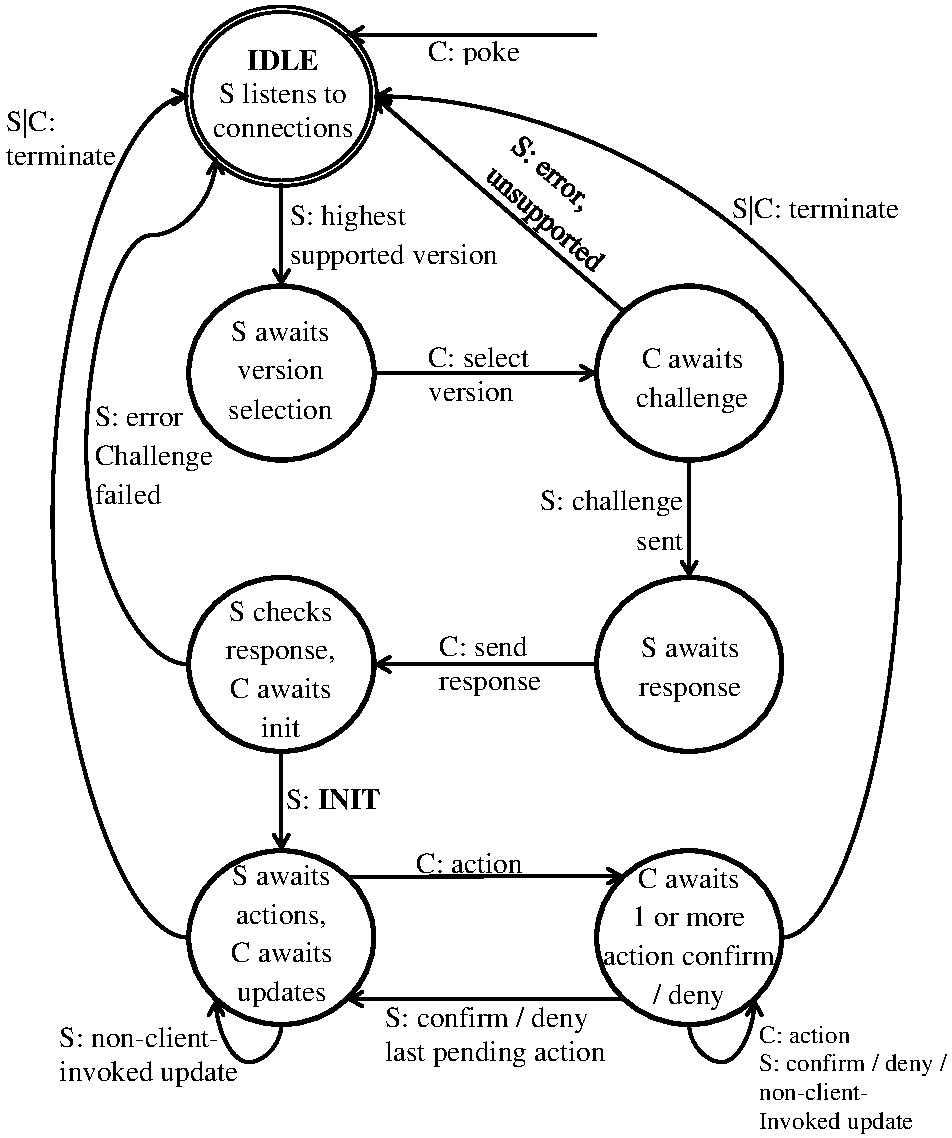
\includegraphics[width=5in]{figures/dfa.pdf}
  \caption{DFA illustration for the RSHC protocol.}
\end{figure}

We chose to use only two states for the asynchronous phase of the protocol for simplicity. However, we can pair a DFA state to each subset of legal messages, which means a state for every configuration of the house: the states of all monitored devices. This approach would yield a number of states exponential in the number of devices, and a correspondence to the states of the application. Since the two-states model is sufficient for representation, it is chosen for the illustration of the protocol.
